
\section{Platform Architecture}

The developed platform has modules that cover the main steps of a metabolomics data analysis workflow, of which the ones focusing on spectral data will be emphasized, as well as modules to handle public and private user's projects. 

A graphical representation of the application's modules structure is shown in \autoref{website}, while the file structure is represented in \autoref{file_structure}.

\begin{figure}[H]
	\centering
	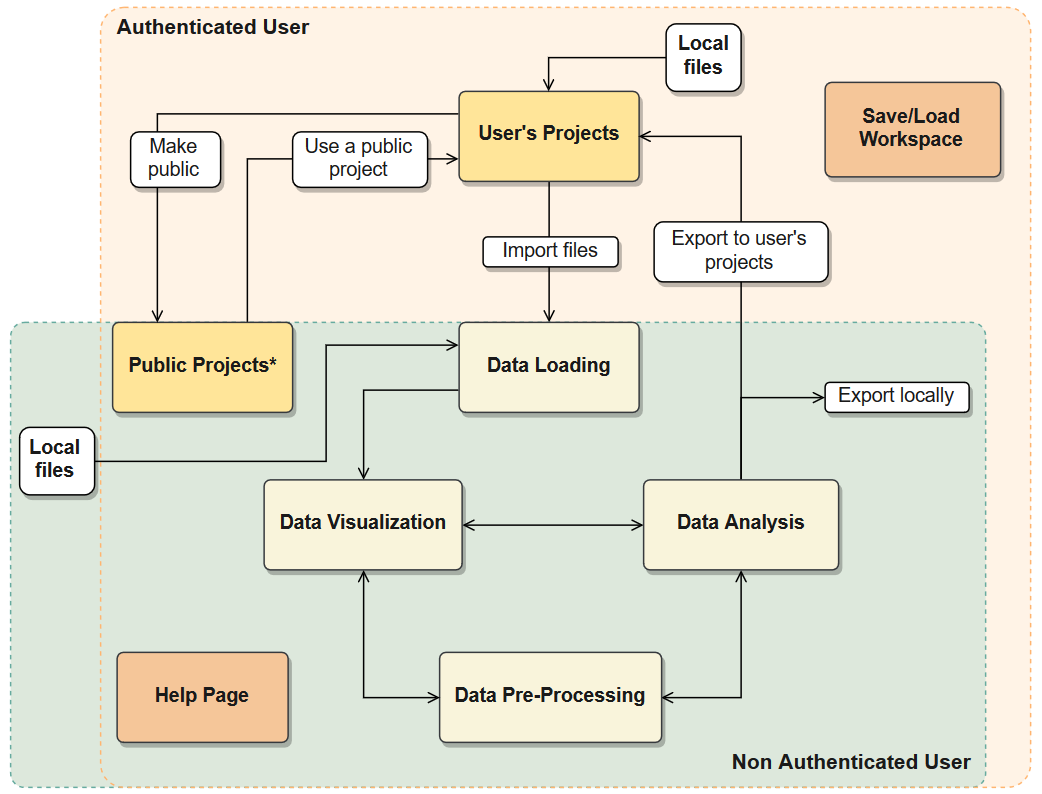
\includegraphics[width=1\linewidth]{Imagens/website_2}
	\caption{Graphical representation of the application's structure, portraying the modules accessible by both non authenticated and authenticated users (green rectangle) or modules accessible only by the latter (yellow rectangle). *Non authenticated users can only view the information contained within the \textit{Public Projects} page, without the possibility to use said information.}
	\label{website}
\end{figure}


The application layout consists in a dashboard with three components: a header, the sidebar and the body, which was created using the R library \textit{shinydashboard}. 

The dashboard header gives access to the \textit{Data Visualization}, \textit{Pre-processing} and \textit{Run Analysis} modules, as well as the \textit{Saving} and \textit{Loading Workspace} options. The header also includes the option to load a project, which is done through the \textit{Choose Files} button if the user is logged in, or through the \textit{New Project} button otherwise. Lastly, the dashboard header also includes a button to handle the authentication of the user and his account options. 


\begin{figure}[H]
	\centering
	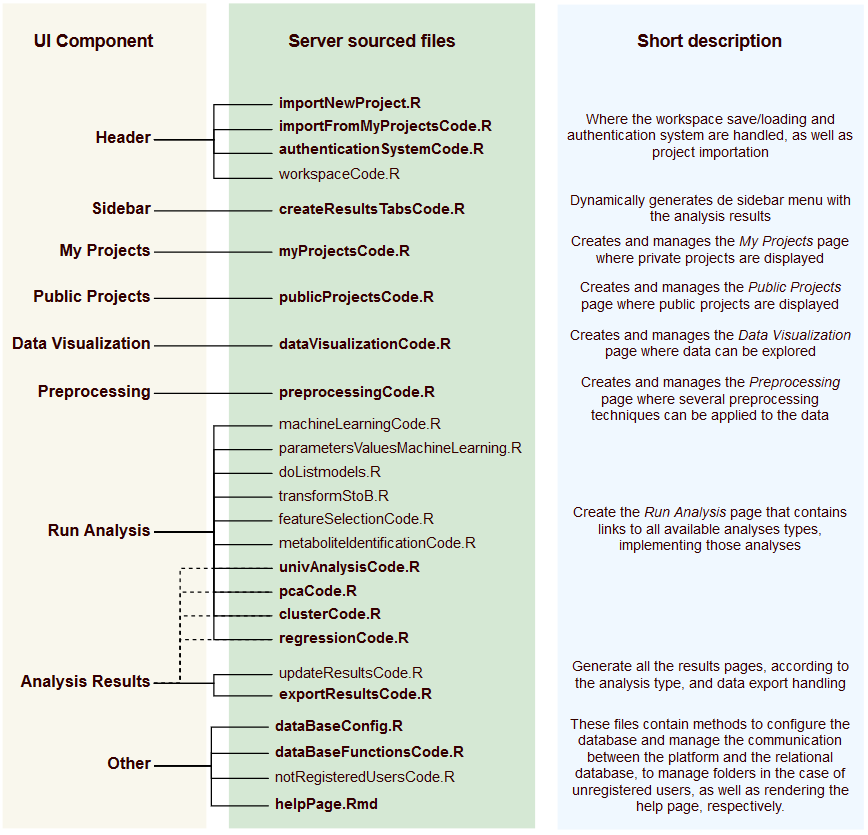
\includegraphics[width=1\linewidth]{Imagens/file_structure}
	\caption{Graphical representation of the application's file structure. The filenames in bold represent the files to which the author of this dissertation greatly or totally contributed to, given the scope of this work.}
	\label{file_structure}
\end{figure}

On the other hand, the dashboard sidebar includes four tabs: the \textit{Home} tab, which represents the main page of the web application; the \textit{My Projects} tab, containing information about the user's stored projects; the \textit{Public Projects} tab where all user's shared projects are shown; and the \textit{HELP} tab that contains helpful information about each feature available on the platform, under the form of text or, in a near future, as tutorial videos. When a project is loaded the current dataset is also shown on the sidebar. The analysis results can be accessed in the \textit{Analysis Results} menu.

The dashboard organization can be viewed in \autoref{webspecmine_home}, where the main page of the web platform is shown. The different modules will be discussed in the following sections. 

\begin{figure}[H]
	\centering
	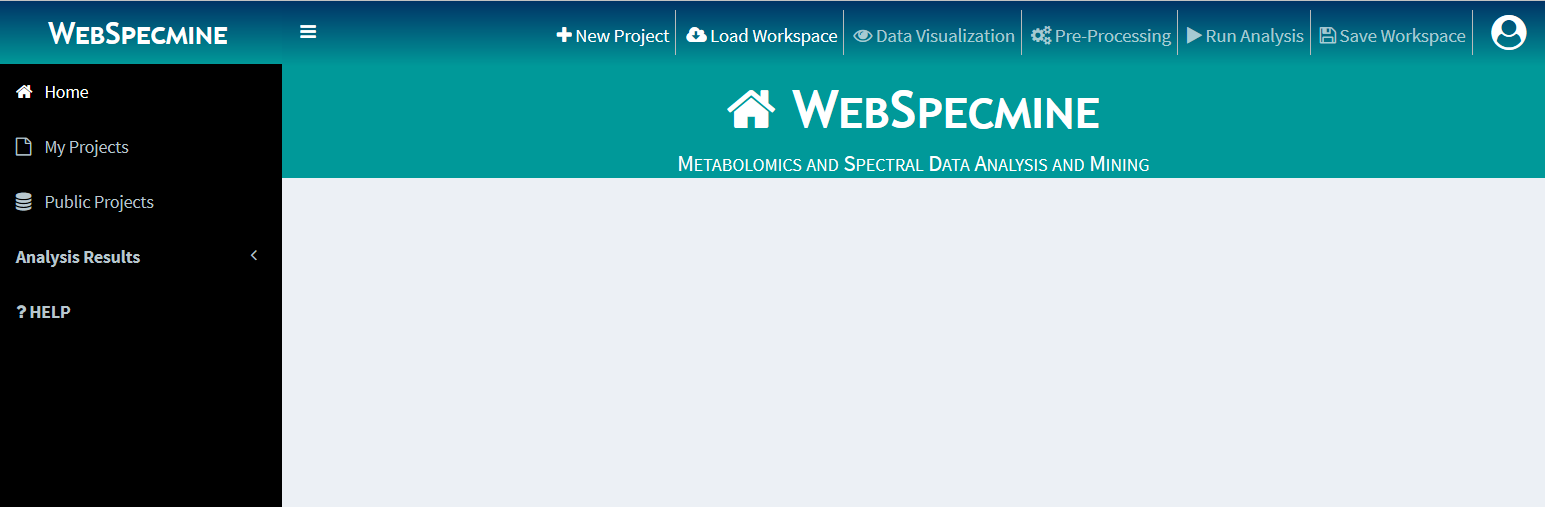
\includegraphics[width=1\linewidth]{Imagens/webspecmine_home}
	\caption{Main page of the web application.}
	\label{webspecmine_home}
\end{figure}


\section{Authentication System}

\begin{wrapfigure}{r}{0.40\textwidth}
	\centering
	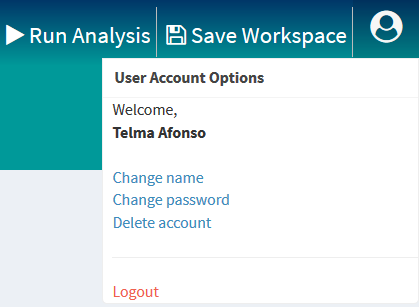
\includegraphics[width=\linewidth]{Imagens/webspecmine_authentication}
	\caption{Authentication menu after successful login (detail).}\label{website_authentication}
\end{wrapfigure}

In the web application, the authentication is made through the \textit{user} button on the upper right corner. Here, the user can either login or register with his e-mail. The password encryption process is explained in \autoref{password}.

Once logged-in, the user has the option to change his name and password, as well as deleting his account, in which case a warning about the account being permanently deleted is shown. The user also has the option to logout, which refreshes the page and the app is set to default values (\autoref{website_authentication}).

%\begin{figure}[h]
%	\centering
%	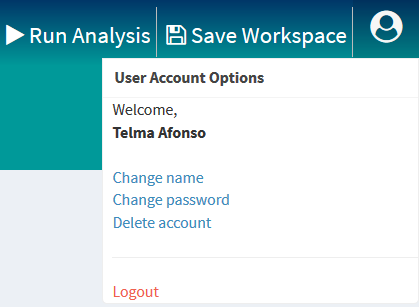
\includegraphics[width=0.6\linewidth]{Imagens/webspecmine_authentication}
%	\caption{Authentication menu after successful login (Zoomed-in).}
%	\label{website_authentication}
%\end{figure}

%\begin{wrapfigure}{r}{2cm}
%	
%	\caption{Authentication menu after successful login (Zoomed-in).}
%	\label{website_authentication}
%	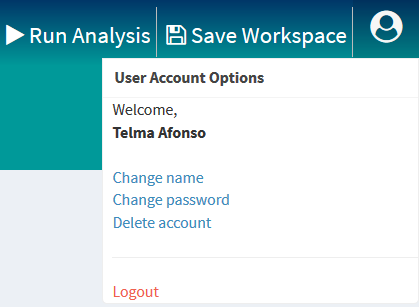
\includegraphics{Imagens/webspecmine_authentication}
%\end{wrapfigure} 



\section{Private and Public Projects}

The modules that handle public and private user's projects are \textit{Public Projects} and \textit{My Projects}, respectively. In this web application, a project is associated with a data folder, which contains sub folders to store one or more datasets that can be of different data types; a metadata folder, which stores one or more metadata files; and a reports folder to store the reports generated during the analysis. A graphical representation of a project's structure is shown in \autoref{project}.

\begin{figure}[h]
	\centering
	\includegraphics[width=0.5\linewidth]{Imagens/project}
	\caption{Graphical representation of a project's structure.}
	\label{project}
\end{figure}

To access the \textit{My Projects} page, the user must be authenticated. Here, all the user's saved projects are displayed, including each project's description, datasets, metadata and report files. 

The user is able to create new projects and data folders for each project and also to edit their information, including the data type in the case of a data folder or name and description in both cases. Both projects and folders can be deleted, as well as the files contained within the folders.

For each data and metadata folder one or multiple files can be uploaded, to be later used in an analysis. When creating a project the user can decide whether or not to make it public, in which case it will be available for every user. The project status can be changed at anytime using the circular button for the effect. All the user's stored files in this module can be viewed or downloaded at any time. A zoomed view of the \textit{My Projects} page with the metadata tab selected is shown in \autoref{webspecmine_myprojs}.

\begin{figure}[h]
	\centering
	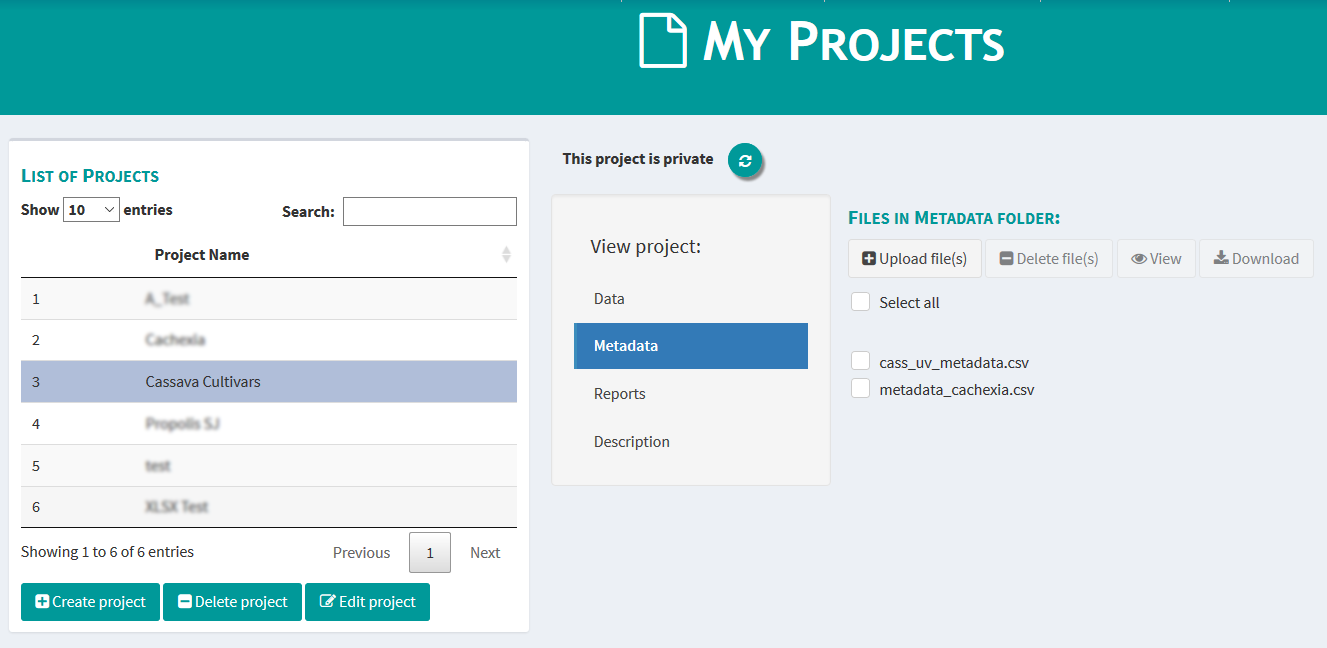
\includegraphics[width=0.9\linewidth]{Imagens/webspecmine_myprojs}
	\caption{Zoomed view over \textit{My Projects} page.}
	\label{webspecmine_myprojs}
\end{figure}

The \textit{Public Projects} module can be accessed without any kind of authentication. Here, all projects that have been made public are displayed in table format, with information about the project name, author and data type. Any project can be imported into the user's private projects collection, given that the user is authenticated and the project itself is not owned by the user nor does he already own a project by that name. Each project in this module has a description, data, metadata and reports files associated, as in the previous module, that can be viewed at any given time. To obtain the latest list of public projects a \textit{refresh} button is provided.

An important feature also present in the web application is the ability to save and load the workspace. This way, all the data and results the user is currently working on can be saved into his account for later use, thus providing the ability to continue the analysis at any given time.

\section{Import Files} \label{import_files}

Before any analysis can be made, the data must be loaded into the web application. This is done by clicking the \textit{Choose Files} or \textit{New Project} buttons on the dashboard header, which depends on whether or not the user is authenticated, respectively.

In the case of being authenticated, a window with three sections opens. These sections are related with the project, data folder and metadata file to be imported from the user's projects. After choosing the correct files a new window with options to create the dataset appears, according to the data type. 

For spectral data, the data options consist in choosing the file type, that is, whether the selected folder has a single CSV file or multiple CSV, JDX, SPC or XLSX files, the field separator character, whether the samples are represented in columns or rows and if the file has row/column headers. Metadata options consist in choosing the field separator character and whether the file has row/column headers. Additionally, a short description of the data and the \textit{x} and \textit{y} axis labels may be provided. 

On the other hand, if the user is not authenticated the files must be instead uploaded directly into the web application. However, the data and metadata options are the same as in the previous case. The \textit{New Project} window for spectral data is shown in \autoref{webspecmine_import}.

\begin{figure}[h]
	\centering
	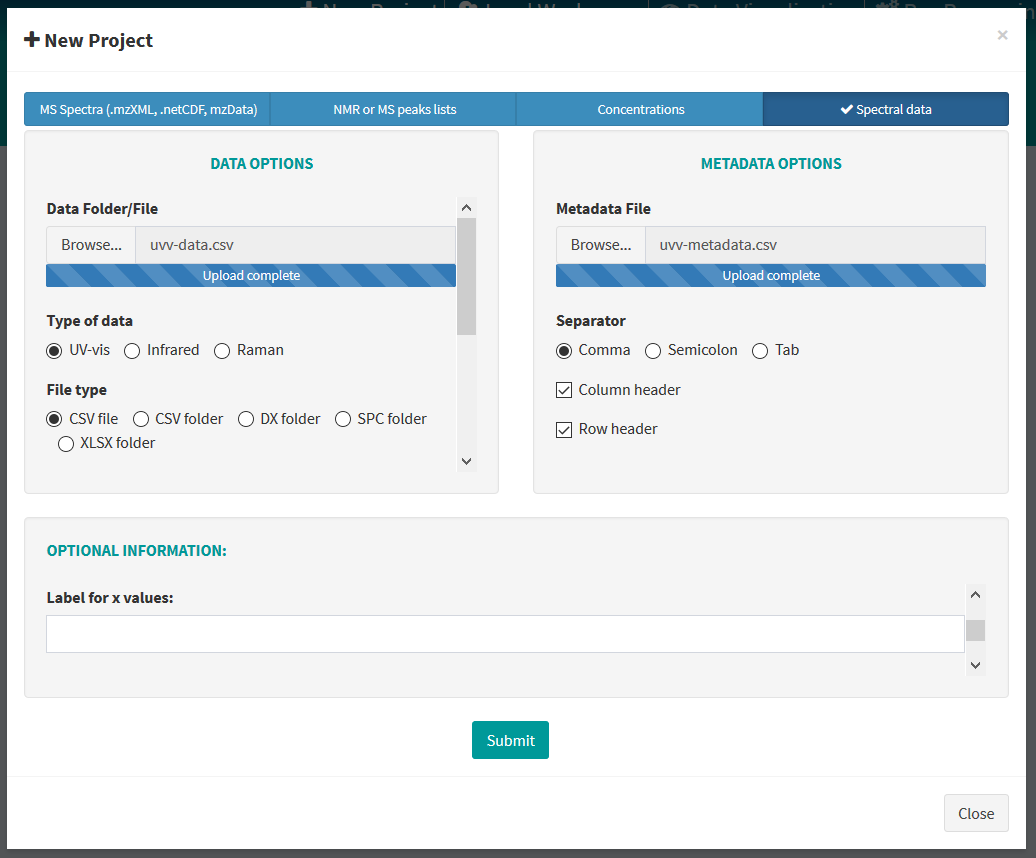
\includegraphics[width=0.8\linewidth]{Imagens/webspecmine_import}
	\caption{Zoomed view over \textit{New Project} window.}
	\label{webspecmine_import}
\end{figure}

In both cases, the \textit{specmine}'s functions used to implement the data reading process are described in \autoref{specmine_functions_data_reading}.


\section{Data Visualization}

When a dataset is loaded, the data and some of its global statistics can be viewed in the \textit{Data Visualization} page. Here, the data and metadata tables, the data summary, a boxplot of the variables and the spectra plot are shown. 

The \textit{Data Summary} tab shows the summary of the loaded dataset, containing the description, type of data, number of samples, data points, metadata variables and missing values, \textit{x} and \textit{y} axis labels, mean, median and range of data values, standard deviation and quantiles of the dataset. The \textit{specmine} function to retrieve the data summary is described in \autoref{specmine_functions_prepocessing}.

In the \textit{Data Table} tab, as the name indicates, a table with all data points is shown, with variables in the rows and samples in the columns. The \textit{Metadata Table}, on the other hand, shows information regarding the metadata, with samples represented in rows and variables in columns. Both tables can be searched for a specific term and ordered by column.

When the loaded dataset is either of the type \gls{nmr}, \gls{ms}, \gls{ir}, \gls{uv} or Raman spectra, an additional tab -- \textit{Spectra Plot} -- is shown, containing the spectra plotted from the dataset, using \textit{specmine}'s \textit{plot\_spectra} function. A number of options are available to adjust the plot, including the metadata variable to color the plot, the samples and the \textit{x} axis range to plot, also including  the option to reverse the \textit{x} axis.  \autoref{data_visualization} shows a zoomed view of the \textit{Spectra Plot} tab in the \textit{Data Visualization} page.

\begin{figure}[h]
	\centering
	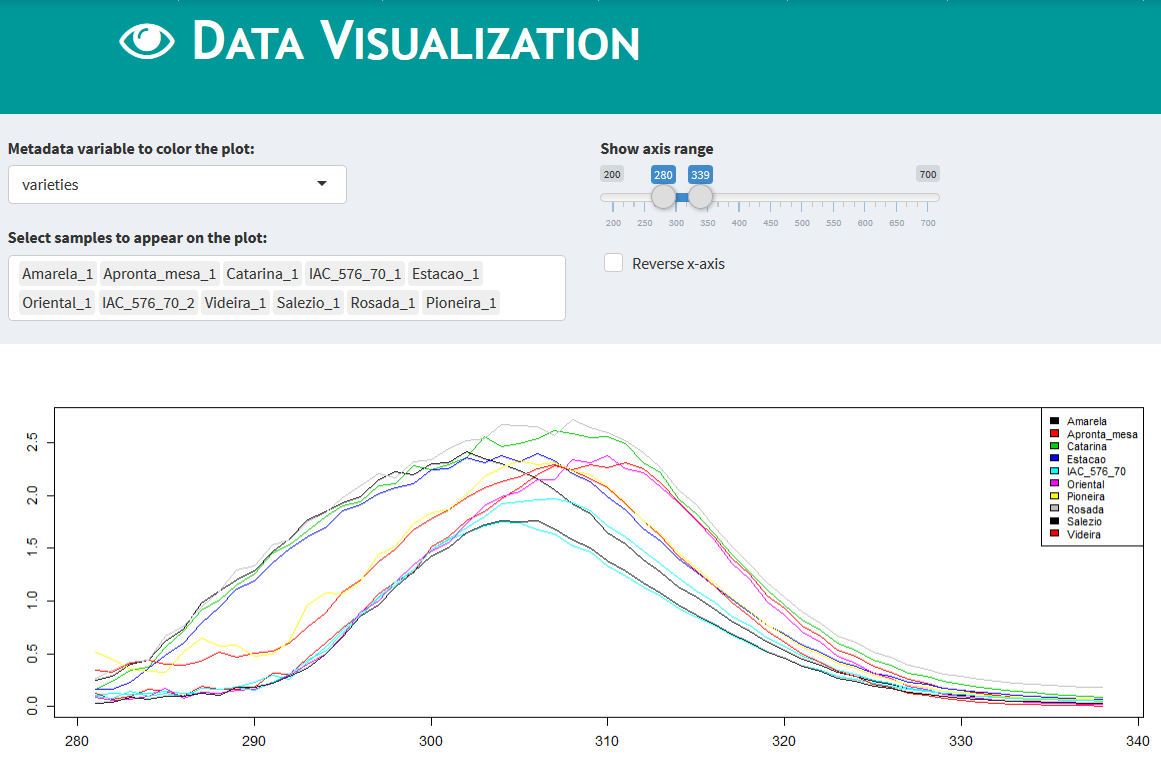
\includegraphics[width=0.9\linewidth]{Imagens/data_visualization}
	\caption{Zoomed view over \textit{Spectra Plot} tab in the \textit{Data Visualization} page.}
	\label{data_visualization}
\end{figure}

Lastly, the \textit{Boxplot of the Variables} tab shows a boxplot that can have from one to the total number of variables plotted, which are selected using a \textit{pickerinput} object from \textit{shinyWidgets} library. The boxplot is plotted using a \textit{specmine} function described in \autoref{specmine_functions_prepocessing}.

An HTML report can be generated with the above information to be either downloaded or saved into the user reports folder of the selected project, in case he is authenticated.



\section{Preprocessing}

On the \textit{Pre-Processing} page, a number of pre-processing approaches can be applied to the data. The page consists in a series of boxes to which a pre-processing technique is assigned to, displayed in two columns format. This way, various techniques can be applied sequentially with a simple mouse click. While some are straightforward to apply, others can be configured with different methods from which to choose from. Some techniques can only be applied to specific types of data or when a condition is met (e.g. missing values can only be treated if the dataset actually has some). After selecting the pre-processing techniques to apply to the data, the user must name the new dataset that is to be created, thus allowing to create multiple versions of the dataset.

A list with all the pre-processing approaches available in the web application and corresponding selectable methods (\textbf{M}), implemented using specmine functions described in \autoref{specmine_functions_prepocessing}, is presented below:


\begin{multicols}{2}
	\begin{itemize}
		\item \textbf{Aggregate samples}
		\item \textbf{Create subset by interval}	
		\item \textbf{Data correction}
		\begin{itemize}
			\item[\textbf{M}] Baseline; background; offset
%			\item[\textbf{F}] \textit{data\_correction}
		\end{itemize}
		\item \textbf{Data normalization}
		\begin{itemize}
			\item[\textbf{M}] Sum; median
%			\item[\textbf{F}] \textit{normalize}
		\end{itemize}
		\item \textbf{Data transformation}
		\begin{itemize}
			\item[\textbf{M}] Logarithmic; cubic root
%			\item[\textbf{F}] \textit{transform\_data}
		\end{itemize}
		\item \textbf{\acrlong{llf}}
		\item \textbf{Factor conversion}
%		\begin{itemize}
%			\item[\textbf{F}] \textit{convert\_to\_factor}
%		\end{itemize}
		\item \textbf{First derivative}
%		\begin{itemize}
%			\item[\textbf{F}] \textit{first\_derivative}
%		\end{itemize}
		\item \textbf{Smoothing interpolation}
		\begin{itemize}
			\item[\textbf{M}] Bin; loess; Savitzky-Golay
%			\item[\textbf{F}] \textit{smoothing\_interpolation}
		\end{itemize}
		\item \textbf{Flat patter filter}
		\begin{itemize}
			\item[\textbf{M}] Interquartile range; relative standard deviation; standard deviation; median absolute deviation; mean; median
%			\item[\textbf{F}] \textit{flat\_pattern\_filter}
		\end{itemize}	
		\item \textbf{Mean centering}
%		\begin{itemize}
%			\item[\textbf{F}] \textit{mean\_centering}
%		\end{itemize}
		\item \textbf{Missing value handling}
		\begin{itemize}
			\item[\textbf{M}] Mean; median; given value; \gls{knn}, linear approximation
%			\item[\textbf{F}] \textit{missingvalues\_imputation}
		\end{itemize}
		\item \textbf{\acrlong{msc}}
%		\begin{itemize}
%			\item[\textbf{F}] \textit{msc\_correction}
%		\end{itemize}	
		\item \textbf{Remove data}
		\item \textbf{Remove data by NAs}
		\begin{itemize}
			\item[\textbf{M}] Value; Percentage; NAs in metadata
			%			\item[\textbf{F}] \textit{scaling}
		\end{itemize}	
		\item \textbf{Scaling}
		\begin{itemize}
			\item[\textbf{M}] Auto; pareto; range
%			\item[\textbf{F}] \textit{scaling}
		\end{itemize}				
	\end{itemize}
\end{multicols}


%These include mean centering (\textit{mean\_centering}), logarithmic and cubic root data transformations (\textit{transform\_data}), scaling with auto, pareto and range methods (\textit{scaling}), baseline, offset and background corrections (\textit{data\_correction}), smoothing interpolation with methods bin, Loess and Savitzky-Golay (\textit{smoothing\_interpolation}), factor conversion (\textit{convert\_to\_factor}), first derivative (\textit{first\_derivative}), \gls{msc} (\textit{msc\_correction}), data normalization with methods sum and median (\textit{normalize}), missing values handling with methods mean, given value, median, \gls{knn} and linear approximation (\textit{missingvalues\_imputation}), and lastly flat pattern filter with methods interquartile range, relative standard deviation, standard deviation, median absolute deviation, mean and median with option to filter by percentage or threshold (\textit{flat\_pattern\_filter}). 

In \autoref{webspecmine_preprocessing}, a zoomed view of the \textit{Pre-Processing} page is shown, where some of the already mentioned methods, such as missing values handling, data transformation, scaling, data correction, subset creation and data removal are emphasized.


\begin{figure}[h]
	\centering
	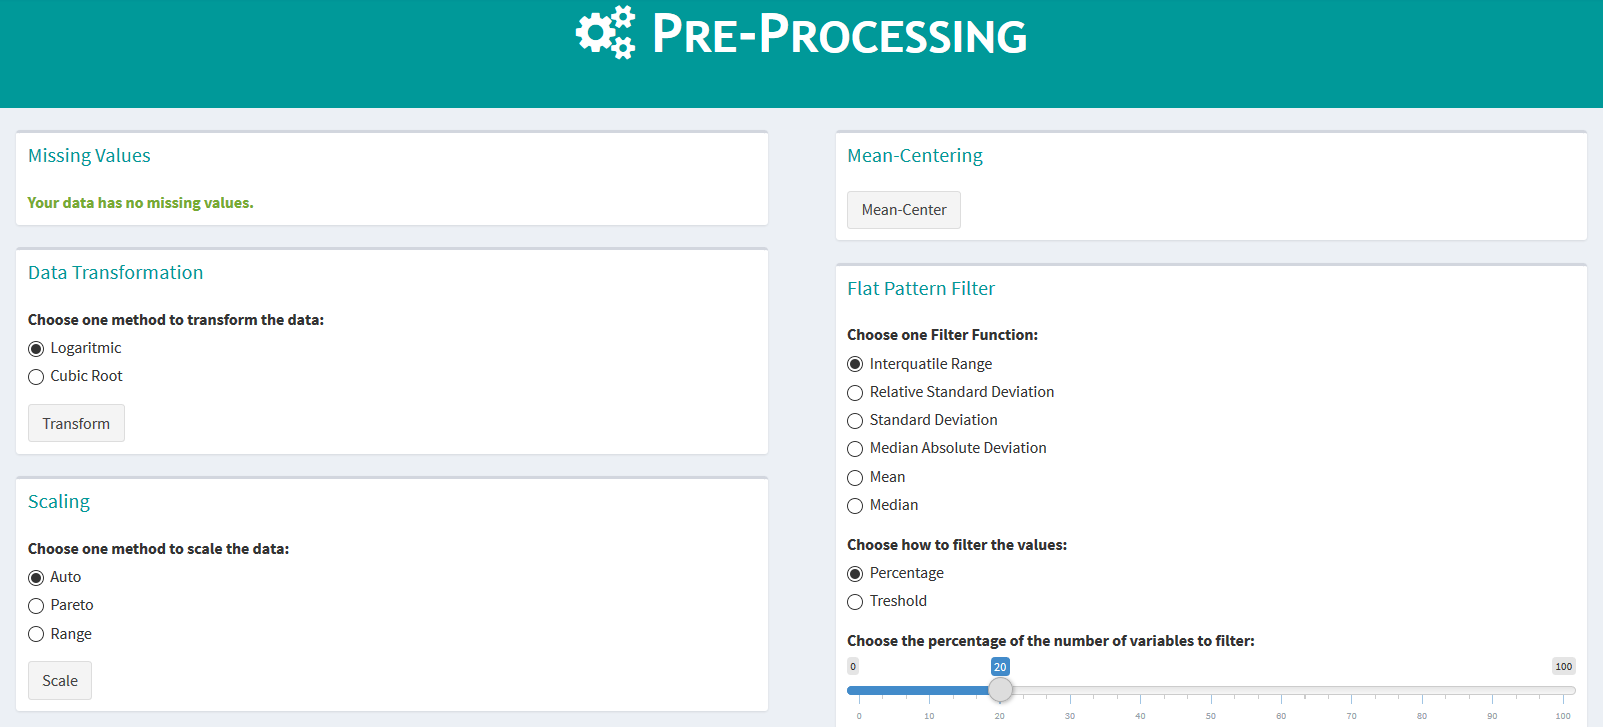
\includegraphics[width=1\linewidth]{Imagens/webspecmine_preprocessing}
	\caption{Zoomed view over \textit{Pre-Processing} page.}
	\label{webspecmine_preprocessing}
\end{figure}



\section{Data Analysis}

Opening the \textit{Run Analysis} page is the first step to perform data analysis using the web application. In this page, each analysis type (or group of analysis) is assigned to a panel with the respective information and a button that leads into the corresponding analyses page, (\autoref{webspecmine_runanalysis}). Currently, there are available univariate analysis such as \gls{anova}, fold change analysis, T-Tests, Kruskal-Wallis and Kolmogorov-Smirnov tests. Unsupervised multivariate analysis include \gls{pca}, hierarchical and k-means clustering and correlation analysis. Other available supervised analyses are machine learning, regression analysis, feature selection and metabolite identification. As already stated, considering the data types emphasized throughout this work (\gls{uv}, \gls{ir} and Raman) are not usually employed in metabolite identification this type of analysis won't be here discussed. 

\begin{figure}[h]
	\centering
	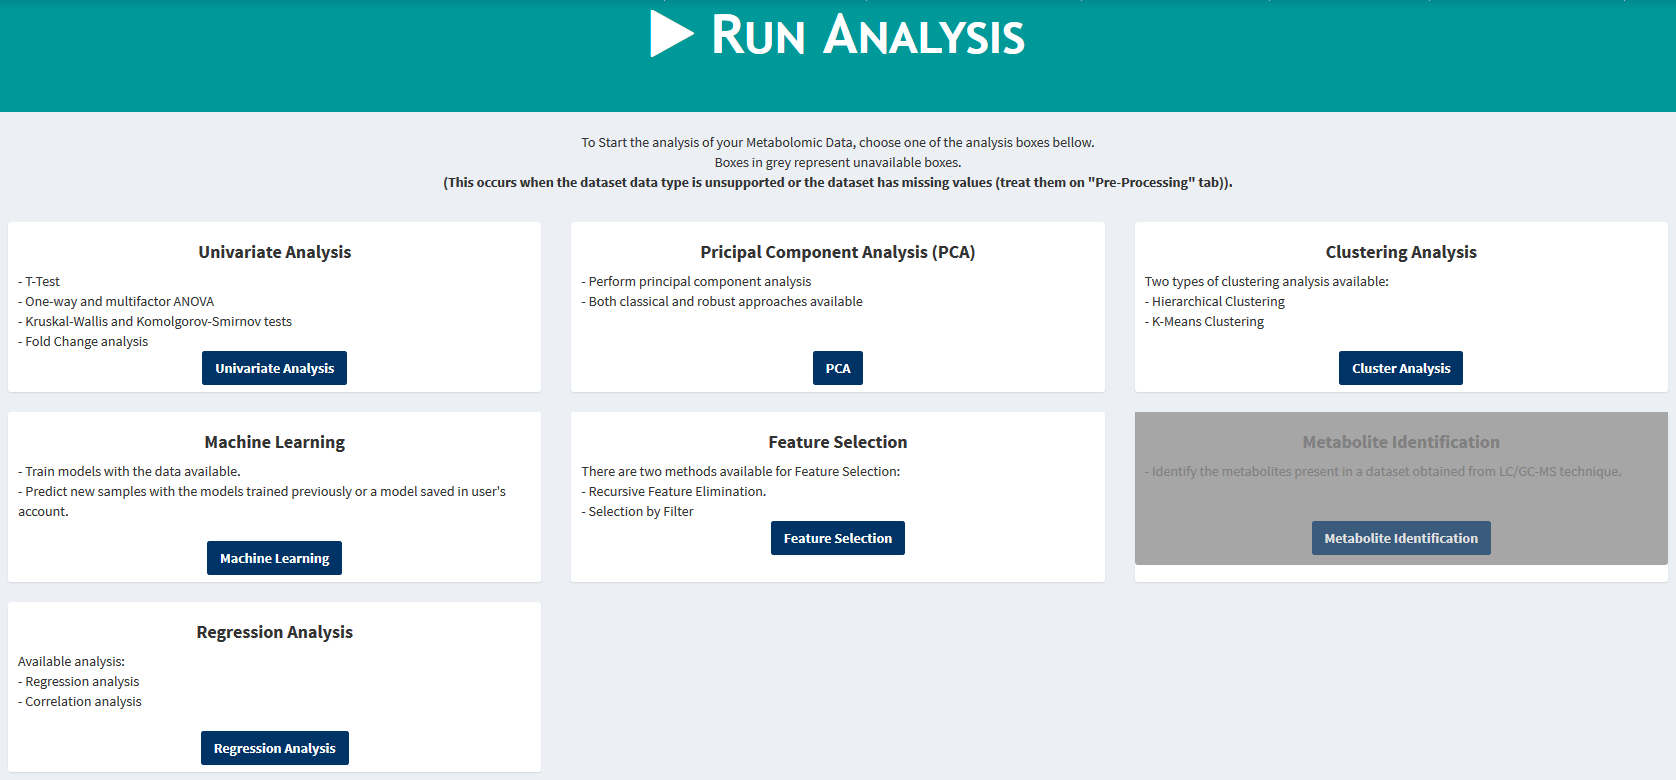
\includegraphics[width=1\linewidth]{Imagens/webspecmine_runanalysis}
	\caption{Zoomed view over the \textit{Run Analysis} page.}
	\label{webspecmine_runanalysis}
\end{figure}

To perform any type of the described methods, a name must be given to the analysis, this being the name that will appear under the corresponding analysis tab in the \textit{Analysis Results} menu on the sidebar. Upon clicking an analysis name, the corresponding results page is opened. Every results page has a round button displayed on the top left corner, which can be clicked to reveal the options used to perform the analysis. It is also important to note that HTML reports and CSV files can be generated with the results at any time, which can then be downloaded and/or saved into the respective project's reports folder. 


\subsection{Univariate Data Analysis}

Regarding univariate data analysis, the web application is able to perform either one-way or multi-factor \gls{anova}, T-Tests, Kruskal-Wallis and Kolmogorov-Smirnov tests, and fold change analysis. These analyses are implemented  using \textit{specmine}'s functions described in \autoref{specmine_functions_analysis}. 

\subsubsection{One-Way Analysis Of Variance}

When performing a one-way \gls{anova} the user must select the metadata variable to use and whether the Tukey's \gls{hsd} test should be applied. Plot options include the p-value threshold and whether the \textit{x} axis should be reversed. In the results page, a table with the p-value, logarithm of p-value, \gls{fdr} and Tukey's test results, if it was selected during the analysis, is shown. The table results are ordered by p-value, but can be also ordered by any other result type and searched for a specific term (\autoref{webspecmine_anova}). For this type of analysis, a plot is also shown, with the negative base 10 logarithm of the p-value represented on the \textit{y} axis and variables represented on the \textit{x} axis. 

\begin{figure}[h]
	\centering
	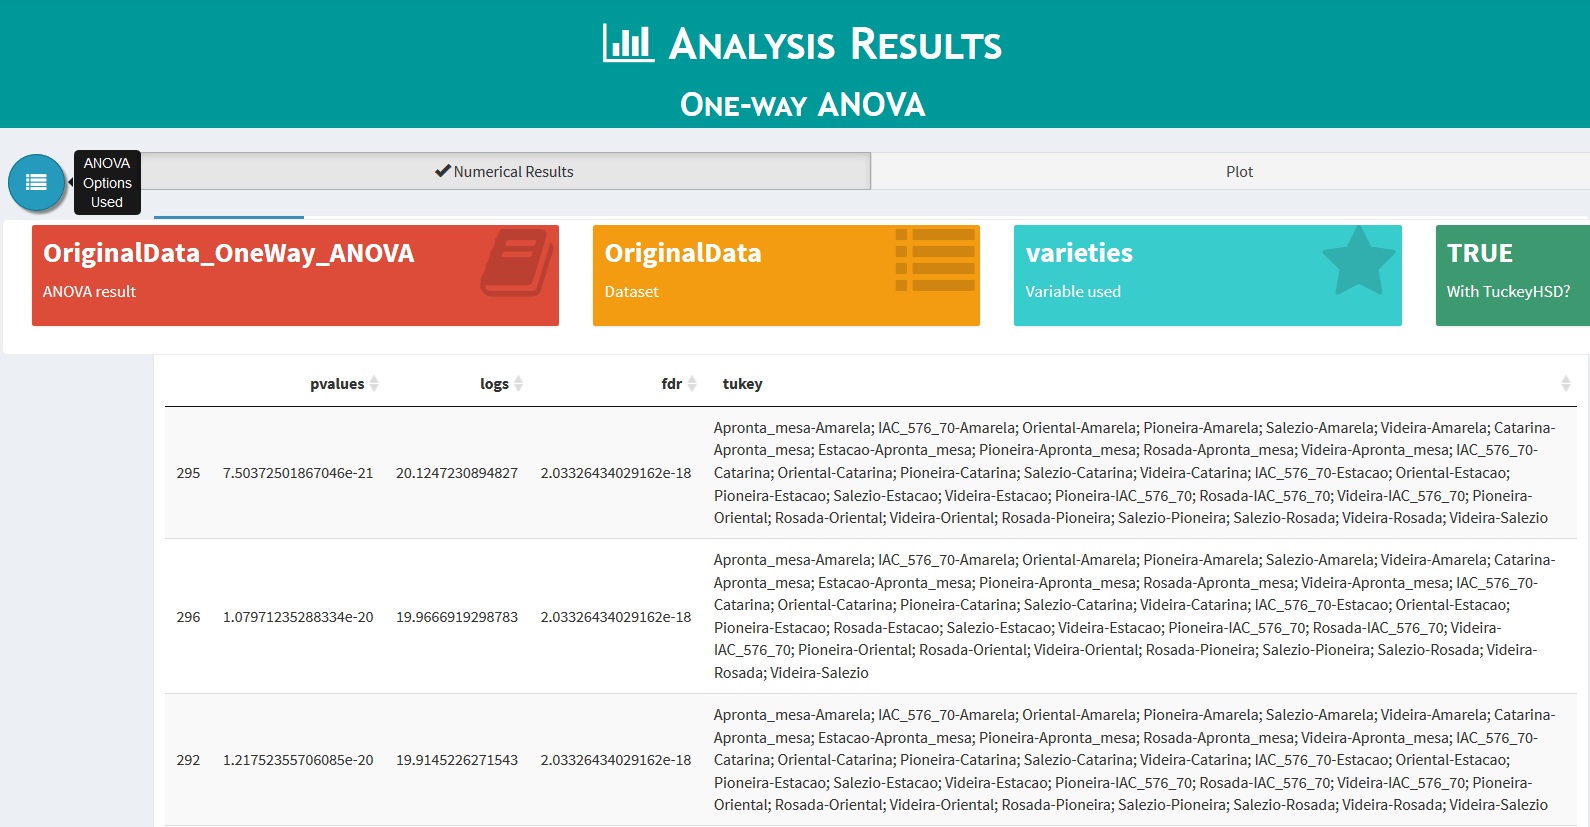
\includegraphics[width=1\linewidth]{Imagens/webspecmine_anova}
	\caption{Zoomed view over \textit{Analysis Results} page for one-way \gls{anova}, showing the numerical results tab and emphasizing the options used for the analysis.}
	\label{webspecmine_anova}
\end{figure}

\subsubsection{Multi-factor Analysis Of Variance}

For the multi-factor \gls{anova}, the metadata variables need to be selected and then a formula, using the selected variables, chosen. The results page for this type of analysis includes a table with the result for each variable on the data, with information regarding the degrees of freedom, sum of squares, mean square, F value, P-value and explained variability.

\subsubsection{T-Tests, Kruskal-Wallis and Kolmogorov-Smirnov Tests}

To run a T-Test, Kruskal-Wallis or Kolmogorov-Smirnov test for each variable from the dataset the user must start by choosing the metadata variable to create the groups of samples as well as the threshold value for the p-value to be considered significant. The results page for the three types of tests are similar, including a table with the p-values, $-log_{\text{10}}$ of the p-values and the \acrlong{fdr}, while also including a plot with variables in the \textit{x} axis and the $-log_{\text{10}}$ of the p-values in the \textit{y} axis.

\subsubsection{Fold Change Analysis}

Two types of fold change analysis can be performed using the web application: either perform the analysis on the entire dataset or over two variables. In the latter case, instead of having the difference of the variables on two groups, the difference of the groups on two variables is calculated. In both cases, the metadata variable to use must be chosen. 

The fold change analysis over the entire dataset requires the user to choose a reference value, namely a class of the metadata variable, while the analysis over two variables requires the user to choose the two variables to use. In the results page, a table with fold change values and the $log_{\text{2}}$ of fold change is shown. It also includes a plot with these $log_{\text{2}}$ of fold change values in the \textit{y} axis and the variable names in the \textit{x} axis, for the analysis over the entire dataset.


\subsection{Linear Regression Analysis}

To perform linear regression analysis, the metadata variables to use must be selected, as well as a formula specifying the model. The results page for this type of analysis includes tables with the p-values, coefficients, r-squared and adjusted r-squared values. It is also possible to plot the linear regression coefficient and the p-values for selected variables, with options to customize the color of the bars and font size.



\subsection{Unsupervised Multivariate Analysis}

Regarding unsupervised multivariate data analysis, the web application is able to perform either classical or robust \gls{pca}, hierarchical and k-means clustering and correlation analysis using \textit{specmine}'s functions described in \autoref{specmine_functions_analysis}.


\subsubsection{Principal Components Analysis}

The simple form of \gls{pca} requires the user to decide if variables are to be scaled and/or centered, while the robust approach allows the centering and scaling methods to be chosen, as well as the number of components. Centering can be done either by mean or median, while scaling methods include standard deviation ratio and mean absolute deviation.

The results pages for both approaches have three tabs: one with the numerical results, another to make the plots and finally a tab where the plots can be visualized. The numerical results tab includes tables with the component importance, the scores matrix and variable loadings for both approaches, while robust \gls{pca} results also include the order of the components.

Available plots are highly customizable, with options that range from selecting the variables to plot to more aesthetic options such as color palette selection (\autoref{webspecmine_pca}A). The available plots in the web application are listed below:

\begin{itemize}
	\item \textbf{Scree plot:} Shows the individual percentages of the explained variance of each principal component and cumulative;
	
	\item \textbf{Pairs plot:} Shows the pairs plot of the scores of the defined principal components, for a chosen variable (\autoref{webspecmine_pca}B);
	
	\item \textbf{Scores plot:} Both 2D and 3D plots that show the scores of two different principal components;
	
	\item \textbf{Biplot:} Plot that displays samples as points, while the variables are displayed either as vectors, linear axes or nonlinear trajectories, considering PC1 and PC2 as axes;
	
	\item \textbf{K-means 2D and pairs plot:} Plots that combine some of the already mentioned plots with k-means results for coloring the points according to the cluster they belong.
			
\end{itemize}


\begin{figure}[h]
	\centering
	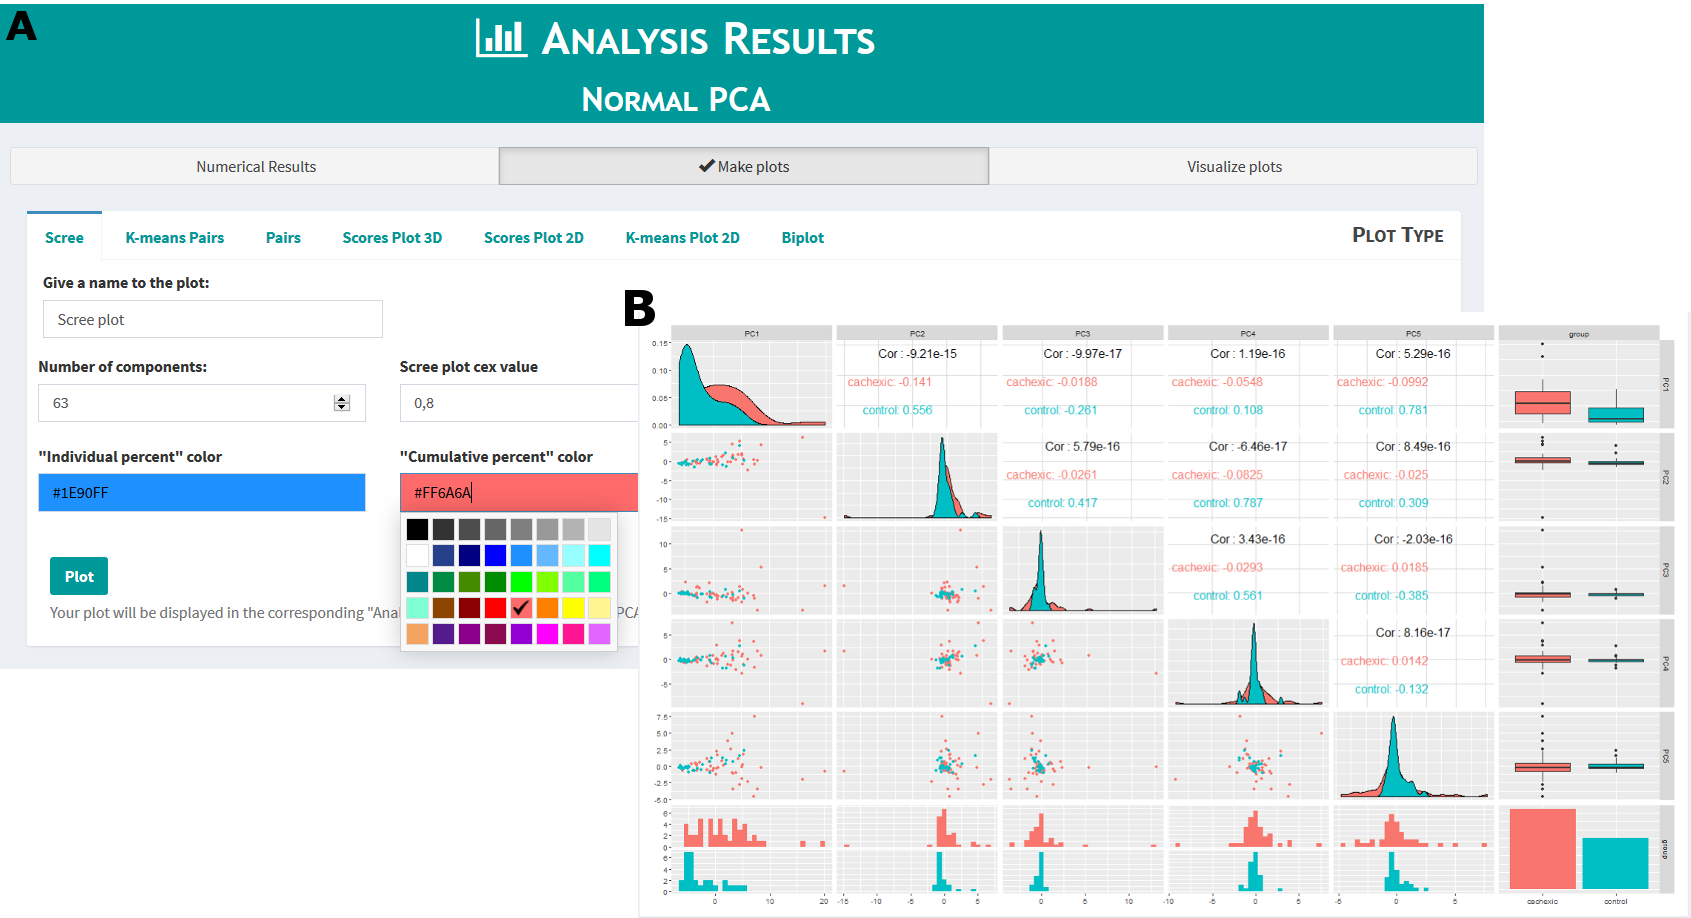
\includegraphics[width=1\linewidth]{Imagens/webspecmine_pca}
	\caption{Zoomed view over the \textit{Analysis Results} page for \gls{pca}, showing the \textit{Make Plots} tab for the scree plot, emphasizing the customizable options (\textbf{A}) and example of a pairs plot made in the web application (\textbf{B}).}
	\label{webspecmine_pca}
\end{figure}


\subsubsection{Clustering Analysis}

Both hierarchical and k-means clustering approaches are available. The former requires the user to select the distance measure (methods include Euclidean, Manhattan, Pearson correlation and Spearman correlation), the agglomeration method (complete, Ward, single, average, McQuitty, median and centroid methods available), and whether to perform the analysis over samples or variables. Additionally, a variable to color the leafs may be chosen. On the other hand, k-means clustering only requires the user to choose the number of clusters and whether to perform the analysis over samples or variables.

The results page for hierarchical clustering analysis includes the resulting dendrogram (\autoref{webspecmine_clustering}), as well as numerical results that comprise heights, order and the labels for the chosen variable to perform the analysis. The dendrogram is plotted using the respective \textit{specmine} function described in \autoref{specmine_functions_analysis}, allowing the dendrogram to show colored leafs, according to the selected variable.

\begin{figure}[h]
	\centering
	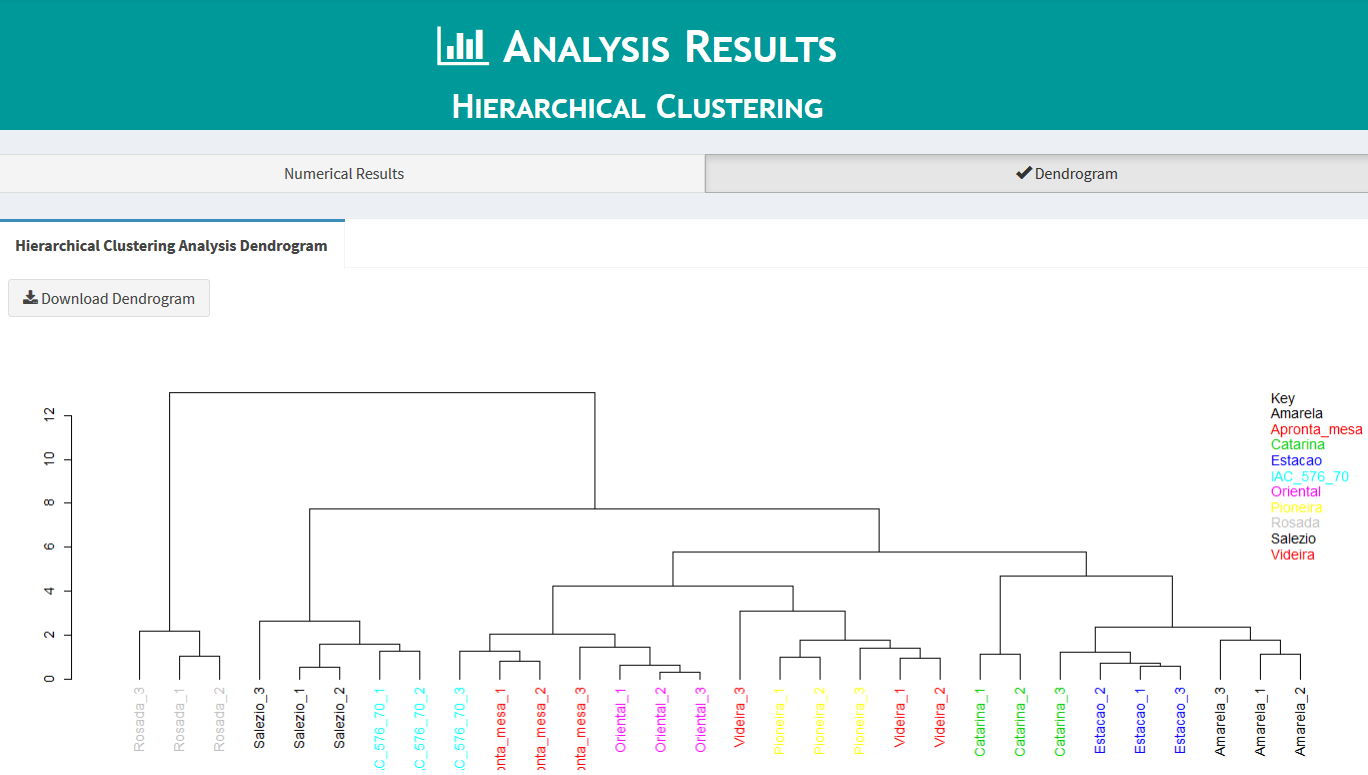
\includegraphics[width=0.9\linewidth]{Imagens/webspecmine_clustering}
	\caption{Zoomed view over \textit{Analysis Results} page for hierarchical clustering, showing the clustering dendrogram.}
	\label{webspecmine_clustering}
\end{figure}

The k-means clustering results page shows information regarding each sample's cluster, the set of samples belonging to each cluster, the centers and the number of samples per cluster. For each cluster a plot is also available, showing in blue the median of the values of the samples in that cluster and in grey all the values of those samples. These plots are implemented using the functions described in \autoref{specmine_functions_analysis}.



\subsubsection{Correlation Analysis}

To perform a correlation analysis between samples or variables the correlation method must be chosen. Three methods are available: Pearson, Kendall and Spearman. The color palette to use in the heatmap is also customizable, with a wide variety of colour gradients available to choose from.

Additionally, a correlations test can be performed over the entire dataset. In such a case, the alternative hypothesis to test must be chosen, and it can be two-sided, greater (for positive association) and less (for negative association).

The results page for this type of analysis includes the correlation matrix and, if a test was performed, the table with the correlation test results. A heatmap is also generated using the correlation matrix, with respective colour scale legend for easier interpretation (\autoref{webspecmine_correlation}).

\begin{figure}[h]
	\centering
	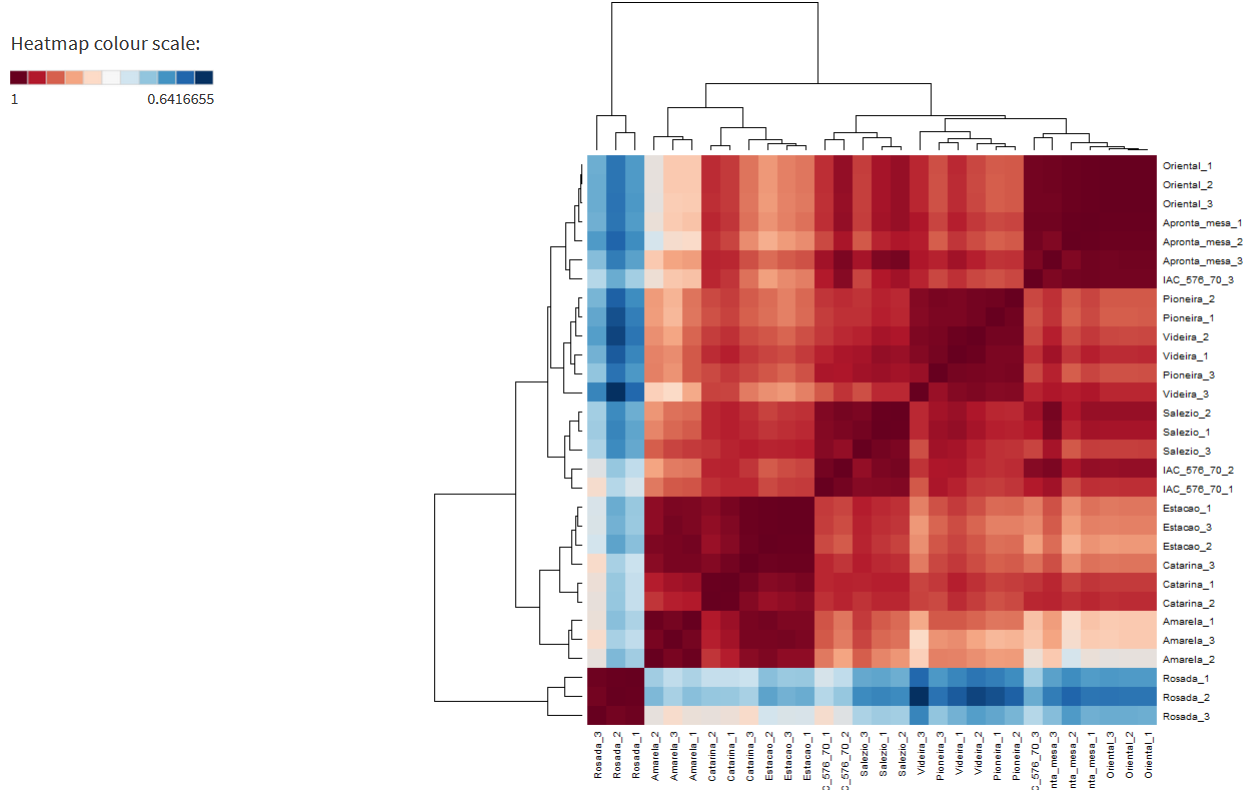
\includegraphics[width=1\linewidth]{Imagens/webspecmine_correlation}
	\caption{Zoomed view over the \textit{Analysis Results} page for correlation analysis, emphasizing the correlation heatmap and respective colour scale.}
	\label{webspecmine_correlation}
\end{figure}



\subsection{Supervised Multivariate Analysis: Machine Learning}

As mentioned before the platform development was shared and this module was not implemented by me, therefore this module will be briefly described.

Regarding machine learning analysis, the web application can perform both model training and prediction of new samples, by implementing \textit{specmine} functions present in \autoref{specmine_functions_machine_learning}. Available models include \gls{pls}, \gls{lda}, decision trees (C4.5-like Trees), rule-based classifier (JRip method), \gls{svm}s with linear kernel, random forests and neural networks. Parameter optimization options are also included. 

%The tunable parameters for the different models are: the number of components for \gls{pls} model, the pruning confidence threshold and minimum instances per leaf for decision tree model, the number of optimizations, folds and weights for rule-based model, the misclassifying influence for \gls{svm} model, the number of variables randomly sampled as candidates at each split for random forests model and the weight decay and number of hidden units for neural network model.

Model validation can be done using resampling, cross-validation, repeated cross-validation, leave-one-out cross-validation and leave group out cross-validation methods. The number of validation folds as well as the metric to test the models performance can also be chosen. These performance test metrics include accuracy and ROC curves.

%The results page for model training shows a table with model performance for every built model, according to the performance metric chosen when performing the analysis. For each trained model, performance metrics such as accuracy, the kappa statistic as well as the standard deviation of the two are shown, alongside the best model parameters and the confusion matrix. The confusion matrix allows to visualize the performance of a model, by showing how many samples were correctly classified or misclassified. The already mentioned performance metrics are also shown for the different number of values tested in each parameter of the models. The overall variable importance as well as its mean are shown in a table for each model, thus completing the results (\autoref{webspecmine_ml}).
%
%\begin{figure}[h]
%	\centering
%	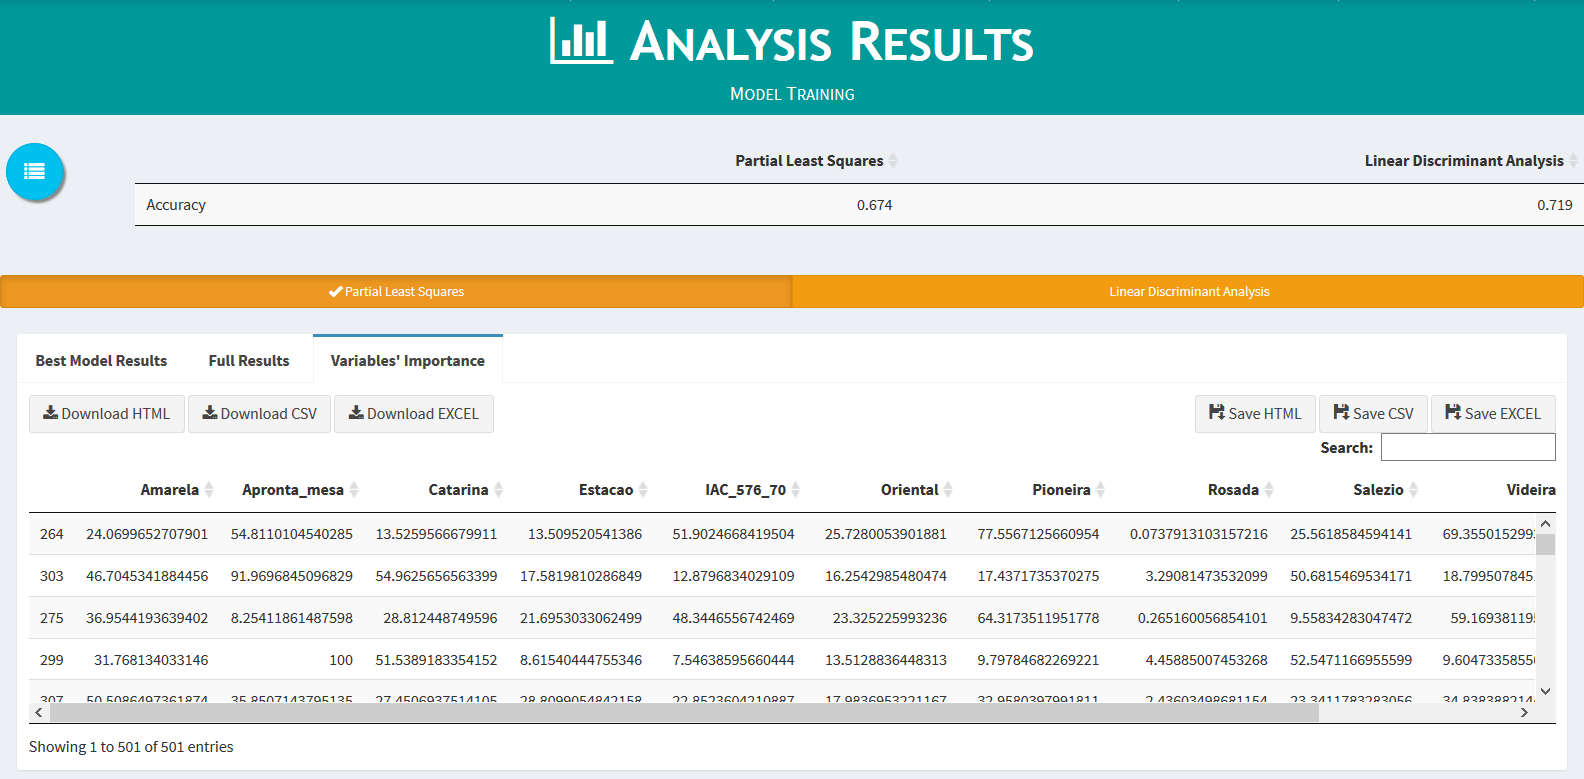
\includegraphics[width=1\linewidth]{Imagens/webspecmine_ml}
%	\caption{Zoomed view over \textit{Analysis Results} page for machine learning \gls{pls} and \gls{lda} model training, emphasizing the results of variable importance.}
%	\label{webspecmine_ml}
%\end{figure}

%To predict new samples, a machine learning model should be previously trained. The user must start by uploading a file containing the dataset with the samples to be predicted, which must be the same dataset used to train the models. The file upload window options are dependent of the data type and are similar to what has been already described in \autoref{import_files}. Upon uploading the file, the samples are further pre-processed similarly to dataset used for model training. Finally one of the trained models is selected and samples can then be predicted.

%Metrics for regression: Root Mean Square Error (RMSE) and the coefficient of determination (R2). Only classification problems?


\subsection{Feature Selection}

Similarly to the previous section, the feature selection module was not developed by me and, therefore, it will be briefly described.

Available feature selection methods include wrappers (\gls{rfe}) and filters. Additionally, the metadata variable where the class to predict is must be chosen, as well as the function for model fitting, prediction and variable importance/filtering, which can be done using random forests, linear regression, bagged trees, \gls{lda} or the Naive-Bayes method. This type of analysis is implemented using \textit{specmine}'s function described in \autoref{specmine_functions_machine_learning}.

%Methods for model validation include bootstrap, cross-validation, repeated cross-validation, leave one out cross-validation and leave group out cross-validation methods. The number of validation folds (or resampling iterations in the case of bootstrap)  and the number of features for each group of test is also selectable.

%The results page for feature selection includes the resampling performance with the already mentioned metrics (accuracy, kappa statistic and their standard deviations), the name of the variables that compose the best subset and the percentage of the variables selected during the resampling. Additionally, a plot with the performance profile across the different subset sizes is also shown.







